\documentclass[1p]{elsarticle_modified}
%\bibliographystyle{elsarticle-num}

%\usepackage[colorlinks]{hyperref}
%\usepackage{abbrmath_seonhwa} %\Abb, \Ascr, \Acal ,\Abf, \Afrak
\usepackage{amsfonts}
\usepackage{amssymb}
\usepackage{amsmath}
\usepackage{amsthm}
\usepackage{scalefnt}
\usepackage{amsbsy}
\usepackage{kotex}
\usepackage{caption}
\usepackage{subfig}
\usepackage{color}
\usepackage{graphicx}
\usepackage{xcolor} %% white, black, red, green, blue, cyan, magenta, yellow
\usepackage{float}
\usepackage{setspace}
\usepackage{hyperref}

\usepackage{tikz}
\usetikzlibrary{arrows}

\usepackage{multirow}
\usepackage{array} % fixed length table
\usepackage{hhline}

%%%%%%%%%%%%%%%%%%%%%
\makeatletter
\renewcommand*\env@matrix[1][\arraystretch]{%
	\edef\arraystretch{#1}%
	\hskip -\arraycolsep
	\let\@ifnextchar\new@ifnextchar
	\array{*\c@MaxMatrixCols c}}
\makeatother %https://tex.stackexchange.com/questions/14071/how-can-i-increase-the-line-spacing-in-a-matrix
%%%%%%%%%%%%%%%

\usepackage[normalem]{ulem}

\newcommand{\msout}[1]{\ifmmode\text{\sout{\ensuremath{#1}}}\else\sout{#1}\fi}
%SOURCE: \msout is \stkout macro in https://tex.stackexchange.com/questions/20609/strikeout-in-math-mode

\newcommand{\cancel}[1]{
	\ifmmode
	{\color{red}\msout{#1}}
	\else
	{\color{red}\sout{#1}}
	\fi
}

\newcommand{\add}[1]{
	{\color{blue}\uwave{#1}}
}

\newcommand{\replace}[2]{
	\ifmmode
	{\color{red}\msout{#1}}{\color{blue}\uwave{#2}}
	\else
	{\color{red}\sout{#1}}{\color{blue}\uwave{#2}}
	\fi
}

\newcommand{\Sol}{\mathcal{S}} %segment
\newcommand{\D}{D} %diagram
\newcommand{\A}{\mathcal{A}} %arc


%%%%%%%%%%%%%%%%%%%%%%%%%%%%%5 test

\def\sl{\operatorname{\textup{SL}}(2,\Cbb)}
\def\psl{\operatorname{\textup{PSL}}(2,\Cbb)}
\def\quan{\mkern 1mu \triangleright \mkern 1mu}

\theoremstyle{definition}
\newtheorem{thm}{Theorem}[section]
\newtheorem{prop}[thm]{Proposition}
\newtheorem{lem}[thm]{Lemma}
\newtheorem{ques}[thm]{Question}
\newtheorem{cor}[thm]{Corollary}
\newtheorem{defn}[thm]{Definition}
\newtheorem{exam}[thm]{Example}
\newtheorem{rmk}[thm]{Remark}
\newtheorem{alg}[thm]{Algorithm}

\newcommand{\I}{\sqrt{-1}}
\begin{document}

%\begin{frontmatter}
%
%\title{Boundary parabolic representations of knots up to 8 crossings}
%
%%% Group authors per affiliation:
%\author{Yunhi Cho} 
%\address{Department of Mathematics, University of Seoul, Seoul, Korea}
%\ead{yhcho@uos.ac.kr}
%
%
%\author{Seonhwa Kim} %\fnref{s_kim}}
%\address{Center for Geometry and Physics, Institute for Basic Science, Pohang, 37673, Korea}
%\ead{ryeona17@ibs.re.kr}
%
%\author{Hyuk Kim}
%\address{Department of Mathematical Sciences, Seoul National University, Seoul 08826, Korea}
%\ead{hyukkim@snu.ac.kr}
%
%\author{Seokbeom Yoon}
%\address{Department of Mathematical Sciences, Seoul National University, Seoul, 08826,  Korea}
%\ead{sbyoon15@snu.ac.kr}
%
%\begin{abstract}
%We find all boundary parabolic representation of knots up to 8 crossings.
%
%\end{abstract}
%\begin{keyword}
%    \MSC[2010] 57M25 
%\end{keyword}
%
%\end{frontmatter}

%\linenumbers
%\tableofcontents
%
\newcommand\colored[1]{\textcolor{white}{\rule[-0.35ex]{0.8em}{1.4ex}}\kern-0.8em\color{red} #1}%
%\newcommand\colored[1]{\textcolor{white}{ #1}\kern-2.17ex	\textcolor{white}{ #1}\kern-1.81ex	\textcolor{white}{ #1}\kern-2.15ex\color{red}#1	}

{\Large $\underline{12a_{0442}~(K12a_{0442})}$}

\setlength{\tabcolsep}{10pt}
\renewcommand{\arraystretch}{1.6}
\vspace{1cm}\begin{tabular}{m{100pt}>{\centering\arraybackslash}m{274pt}}
\multirow{5}{120pt}{
	\centering
	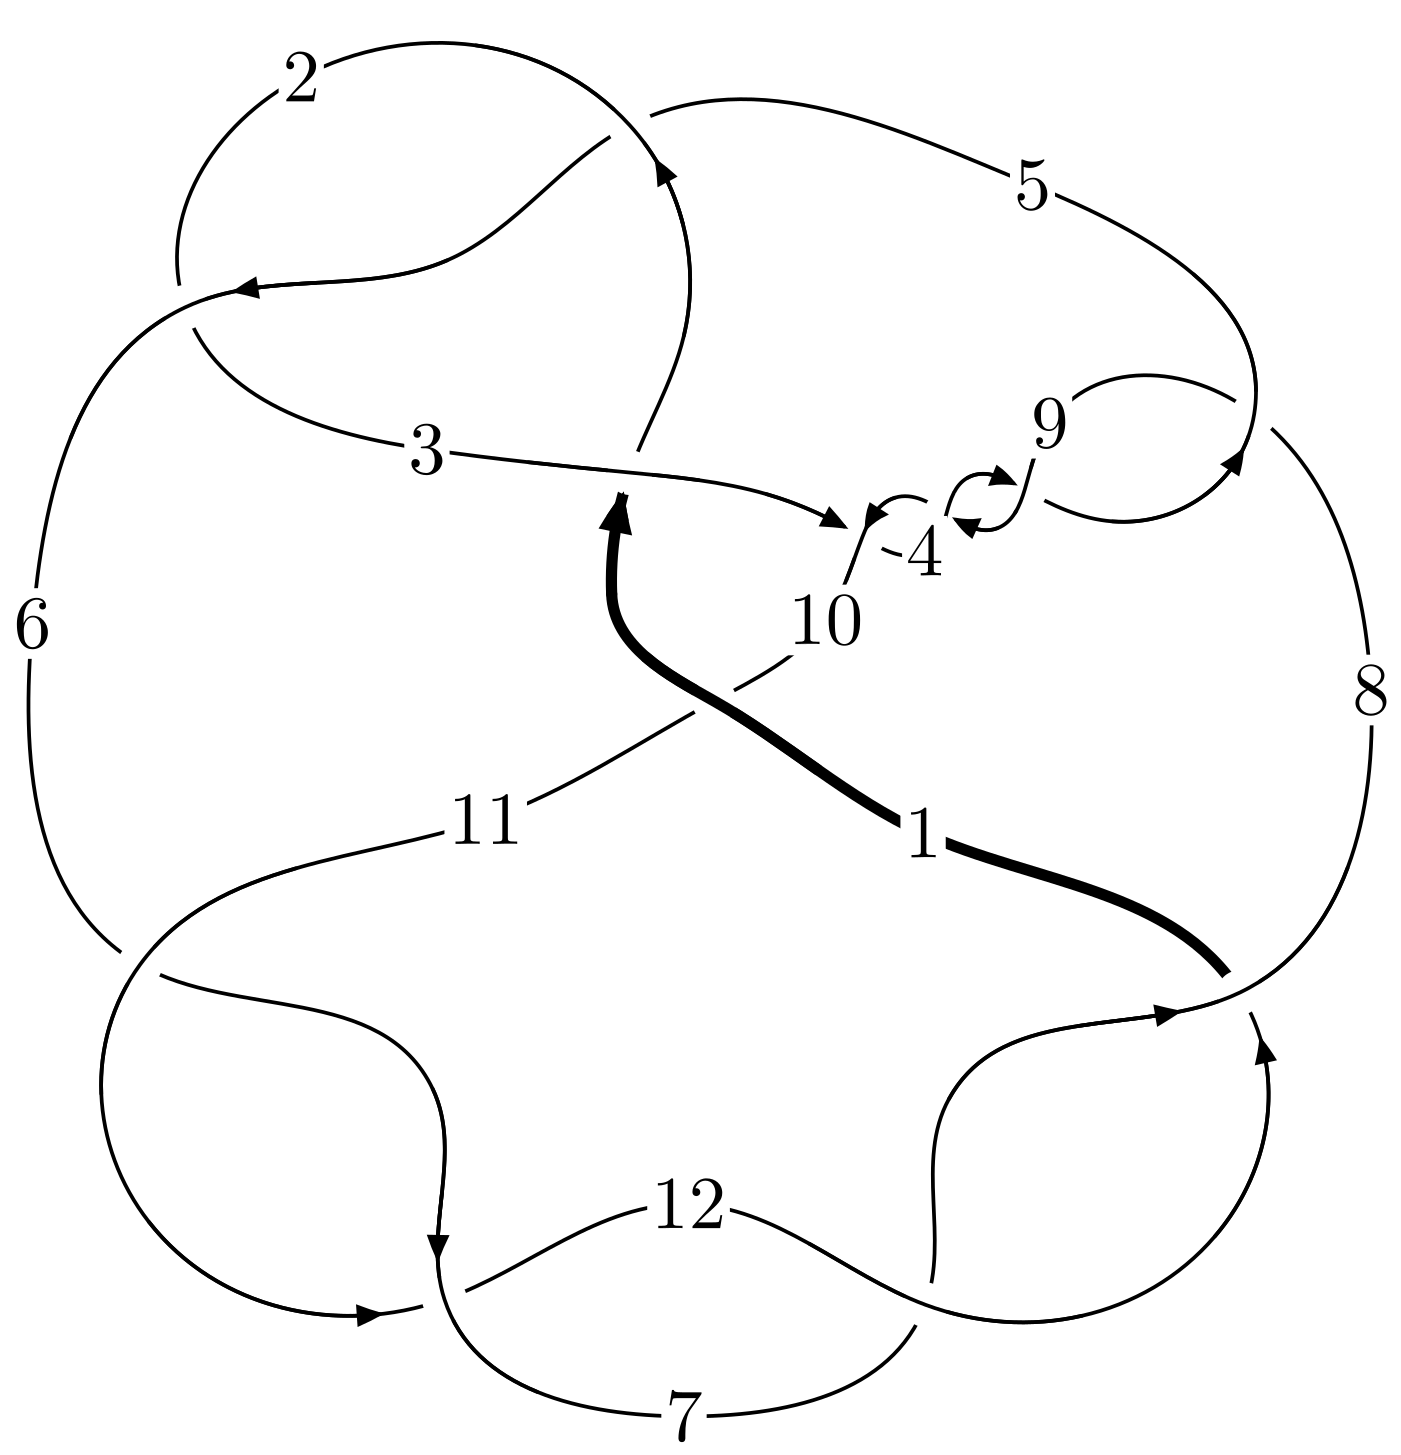
\includegraphics[width=112pt]{../../../GIT/diagram.site/Diagrams/png/1243_12a_0442.png}\\
\ \ \ A knot diagram\footnotemark}&
\allowdisplaybreaks
\textbf{Linearized knot diagam} \\
\cline{2-2}
 &
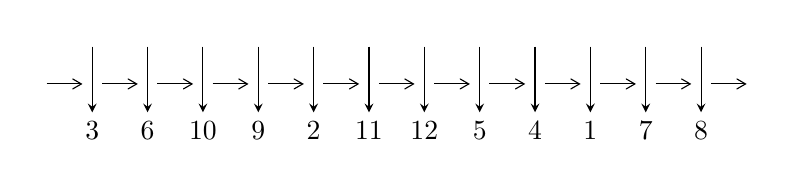
\begin{tikzpicture}[x=20pt, y=17pt]
	% nodes
	\node (C0) at (0, 0) {};
	\node (C1) at (1, 0) {};
	\node (C1U) at (1, +1) {};
	\node (C1D) at (1, -1) {3};

	\node (C2) at (2, 0) {};
	\node (C2U) at (2, +1) {};
	\node (C2D) at (2, -1) {6};

	\node (C3) at (3, 0) {};
	\node (C3U) at (3, +1) {};
	\node (C3D) at (3, -1) {10};

	\node (C4) at (4, 0) {};
	\node (C4U) at (4, +1) {};
	\node (C4D) at (4, -1) {9};

	\node (C5) at (5, 0) {};
	\node (C5U) at (5, +1) {};
	\node (C5D) at (5, -1) {2};

	\node (C6) at (6, 0) {};
	\node (C6U) at (6, +1) {};
	\node (C6D) at (6, -1) {11};

	\node (C7) at (7, 0) {};
	\node (C7U) at (7, +1) {};
	\node (C7D) at (7, -1) {12};

	\node (C8) at (8, 0) {};
	\node (C8U) at (8, +1) {};
	\node (C8D) at (8, -1) {5};

	\node (C9) at (9, 0) {};
	\node (C9U) at (9, +1) {};
	\node (C9D) at (9, -1) {4};

	\node (C10) at (10, 0) {};
	\node (C10U) at (10, +1) {};
	\node (C10D) at (10, -1) {1};

	\node (C11) at (11, 0) {};
	\node (C11U) at (11, +1) {};
	\node (C11D) at (11, -1) {7};

	\node (C12) at (12, 0) {};
	\node (C12U) at (12, +1) {};
	\node (C12D) at (12, -1) {8};
	\node (C13) at (13, 0) {};

	% arrows
	\draw[->,>={angle 60}]
	(C0) edge (C1) (C1) edge (C2) (C2) edge (C3) (C3) edge (C4) (C4) edge (C5) (C5) edge (C6) (C6) edge (C7) (C7) edge (C8) (C8) edge (C9) (C9) edge (C10) (C10) edge (C11) (C11) edge (C12) (C12) edge (C13) ;	\draw[->,>=stealth]
	(C1U) edge (C1D) (C2U) edge (C2D) (C3U) edge (C3D) (C4U) edge (C4D) (C5U) edge (C5D) (C6U) edge (C6D) (C7U) edge (C7D) (C8U) edge (C8D) (C9U) edge (C9D) (C10U) edge (C10D) (C11U) edge (C11D) (C12U) edge (C12D) ;
	\end{tikzpicture} \\
\hhline{~~} \\& 
\textbf{Solving Sequence} \\ \cline{2-2} 
 &
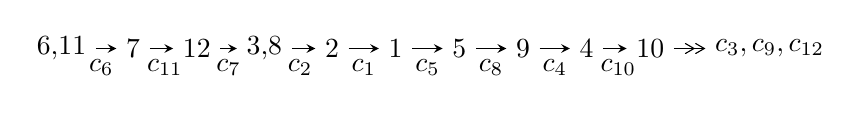
\begin{tikzpicture}[x=23pt, y=7pt]
	% node
	\node (A0) at (-1/8, 0) {6,11};
	\node (A1) at (1, 0) {7};
	\node (A2) at (2, 0) {12};
	\node (A3) at (49/16, 0) {3,8};
	\node (A4) at (33/8, 0) {2};
	\node (A5) at (41/8, 0) {1};
	\node (A6) at (49/8, 0) {5};
	\node (A7) at (57/8, 0) {9};
	\node (A8) at (65/8, 0) {4};
	\node (A9) at (73/8, 0) {10};
	\node (C1) at (1/2, -1) {$c_{6}$};
	\node (C2) at (3/2, -1) {$c_{11}$};
	\node (C3) at (5/2, -1) {$c_{7}$};
	\node (C4) at (29/8, -1) {$c_{2}$};
	\node (C5) at (37/8, -1) {$c_{1}$};
	\node (C6) at (45/8, -1) {$c_{5}$};
	\node (C7) at (53/8, -1) {$c_{8}$};
	\node (C8) at (61/8, -1) {$c_{4}$};
	\node (C9) at (69/8, -1) {$c_{10}$};
	\node (A10) at (11, 0) {$c_{3},c_{9},c_{12}$};

	% edge
	\draw[->,>=stealth]	
	(A0) edge (A1) (A1) edge (A2) (A2) edge (A3) (A3) edge (A4) (A4) edge (A5) (A5) edge (A6) (A6) edge (A7) (A7) edge (A8) (A8) edge (A9) ;
	\draw[->>,>={angle 60}]	
	(A9) edge (A10);
\end{tikzpicture} \\ 

\end{tabular} \\

\footnotetext{
The image of knot diagram is generated by the software ``\textbf{Draw programme}" developed by Andrew Bartholomew(\url{http://www.layer8.co.uk/maths/draw/index.htm\#Running-draw}), where we modified some parts for our purpose(\url{https://github.com/CATsTAILs/LinksPainter}).
}\phantom \\ \newline 
\centering \textbf{Ideals for irreducible components\footnotemark of $X_{\text{par}}$} 
 
\begin{align*}
I^u_{1}&=\langle 
-1.34896\times10^{18} u^{56}+2.07087\times10^{18} u^{55}+\cdots+5.37832\times10^{18} b+3.89959\times10^{18},\\
\phantom{I^u_{1}}&\phantom{= \langle  }1.80814\times10^{19} u^{56}-2.72100\times10^{19} u^{55}+\cdots+3.22699\times10^{19} a-1.14340\times10^{20},\;u^{57}-2 u^{56}+\cdots+3 u+3\rangle \\
I^u_{2}&=\langle 
b+1,\;a+1,\;u^2+u-1\rangle \\
I^u_{3}&=\langle 
b-1,\;a^2-2 a-2 u+5,\;u^2- u-1\rangle \\
\\
\end{align*}
\raggedright * 3 irreducible components of $\dim_{\mathbb{C}}=0$, with total 63 representations.\\
\footnotetext{All coefficients of polynomials are rational numbers. But the coefficients are sometimes approximated in decimal forms when there is not enough margin.}
\newpage
\renewcommand{\arraystretch}{1}
\centering \section*{I. $I^u_{1}= \langle -1.35\times10^{18} u^{56}+2.07\times10^{18} u^{55}+\cdots+5.38\times10^{18} b+3.90\times10^{18},\;1.81\times10^{19} u^{56}-2.72\times10^{19} u^{55}+\cdots+3.23\times10^{19} a-1.14\times10^{20},\;u^{57}-2 u^{56}+\cdots+3 u+3 \rangle$}
\flushleft \textbf{(i) Arc colorings}\\
\begin{tabular}{m{7pt} m{180pt} m{7pt} m{180pt} }
\flushright $a_{6}=$&$\begin{pmatrix}1\\0\end{pmatrix}$ \\
\flushright $a_{11}=$&$\begin{pmatrix}0\\u\end{pmatrix}$ \\
\flushright $a_{7}=$&$\begin{pmatrix}1\\u^2\end{pmatrix}$ \\
\flushright $a_{12}=$&$\begin{pmatrix}- u\\- u^3+u\end{pmatrix}$ \\
\flushright $a_{3}=$&$\begin{pmatrix}-0.560318 u^{56}+0.843200 u^{55}+\cdots+3.40907 u+3.54324\\0.250815 u^{56}-0.385040 u^{55}+\cdots-0.856790 u-0.725058\end{pmatrix}$ \\
\flushright $a_{8}=$&$\begin{pmatrix}- u^2+1\\- u^4+2 u^2\end{pmatrix}$ \\
\flushright $a_{2}=$&$\begin{pmatrix}-0.309503 u^{56}+0.458160 u^{55}+\cdots+2.55228 u+2.81818\\0.250815 u^{56}-0.385040 u^{55}+\cdots-0.856790 u-0.725058\end{pmatrix}$ \\
\flushright $a_{1}=$&$\begin{pmatrix}u^3-2 u\\u^5-3 u^3+u\end{pmatrix}$ \\
\flushright $a_{5}=$&$\begin{pmatrix}0.171913 u^{56}-0.402348 u^{55}+\cdots-5.30776 u-1.55172\\-0.0224250 u^{56}+0.0733178 u^{55}+\cdots+1.08954 u-0.313317\end{pmatrix}$ \\
\flushright $a_{9}=$&$\begin{pmatrix}-1.20094 u^{56}+0.0915331 u^{55}+\cdots+12.1379 u+5.33793\\-0.604807 u^{56}-0.136946 u^{55}+\cdots-0.482139 u+1.18193\end{pmatrix}$ \\
\flushright $a_{4}=$&$\begin{pmatrix}-0.837757 u^{56}+1.11941 u^{55}+\cdots+4.97460 u+4.32404\\0.144564 u^{56}-0.142864 u^{55}+\cdots+0.629938 u-0.344274\end{pmatrix}$ \\
\flushright $a_{10}=$&$\begin{pmatrix}u^7-4 u^5+4 u^3\\u^9-5 u^7+7 u^5-2 u^3+u\end{pmatrix}$\\&\end{tabular}
\flushleft \textbf{(ii) Obstruction class $= -1$}\\~\\
\flushleft \textbf{(iii) Cusp Shapes $= -\frac{826313162299306861}{5378323049132608541} u^{56}-\frac{1448839852347394239}{5378323049132608541} u^{55}+\cdots+\frac{11912765712166984528}{5378323049132608541} u-\frac{107418126212947908801}{5378323049132608541}$}\\~\\
\newpage\renewcommand{\arraystretch}{1}
\flushleft \textbf{(iv) u-Polynomials at the component}\newline \\
\begin{tabular}{m{50pt}|m{274pt}}
Crossings & \hspace{64pt}u-Polynomials at each crossing \\
\hline $$\begin{aligned}c_{1}\end{aligned}$$&$\begin{aligned}
&u^{57}+27 u^{56}+\cdots+3644 u+121
\end{aligned}$\\
\hline $$\begin{aligned}c_{2},c_{5}\end{aligned}$$&$\begin{aligned}
&u^{57}+3 u^{56}+\cdots+50 u+11
\end{aligned}$\\
\hline $$\begin{aligned}c_{3},c_{4},c_{8}\\c_{9}\end{aligned}$$&$\begin{aligned}
&u^{57}+u^{56}+\cdots+16 u+4
\end{aligned}$\\
\hline $$\begin{aligned}c_{6},c_{7},c_{11}\\c_{12}\end{aligned}$$&$\begin{aligned}
&u^{57}-2 u^{56}+\cdots+3 u+3
\end{aligned}$\\
\hline $$\begin{aligned}c_{10}\end{aligned}$$&$\begin{aligned}
&u^{57}-14 u^{56}+\cdots-681 u+369
\end{aligned}$\\
\hline
\end{tabular}\\~\\
\newpage\renewcommand{\arraystretch}{1}
\flushleft \textbf{(v) Riley Polynomials at the component}\newline \\
\begin{tabular}{m{50pt}|m{274pt}}
Crossings & \hspace{64pt}Riley Polynomials at each crossing \\
\hline $$\begin{aligned}c_{1}\end{aligned}$$&$\begin{aligned}
&y^{57}+13 y^{56}+\cdots+4124360 y-14641
\end{aligned}$\\
\hline $$\begin{aligned}c_{2},c_{5}\end{aligned}$$&$\begin{aligned}
&y^{57}-27 y^{56}+\cdots+3644 y-121
\end{aligned}$\\
\hline $$\begin{aligned}c_{3},c_{4},c_{8}\\c_{9}\end{aligned}$$&$\begin{aligned}
&y^{57}+67 y^{56}+\cdots-64 y-16
\end{aligned}$\\
\hline $$\begin{aligned}c_{6},c_{7},c_{11}\\c_{12}\end{aligned}$$&$\begin{aligned}
&y^{57}-66 y^{56}+\cdots+183 y-9
\end{aligned}$\\
\hline $$\begin{aligned}c_{10}\end{aligned}$$&$\begin{aligned}
&y^{57}+6 y^{56}+\cdots+3023883 y-136161
\end{aligned}$\\
\hline
\end{tabular}\\~\\
\newpage\flushleft \textbf{(vi) Complex Volumes and Cusp Shapes}
$$\begin{array}{c|c|c}  
\text{Solutions to }I^u_{1}& \I (\text{vol} + \sqrt{-1}CS) & \text{Cusp shape}\\
 \hline 
\begin{aligned}
u &= -0.704131 + 0.589103 I \\
a &= -0.55492 - 1.95508 I \\
b &= -1.137580 + 0.679596 I\end{aligned}
 & \phantom{-}8.22701 + 10.27850 I & -9.75435 - 7.77331 I \\ \hline\begin{aligned}
u &= -0.704131 - 0.589103 I \\
a &= -0.55492 + 1.95508 I \\
b &= -1.137580 - 0.679596 I\end{aligned}
 & \phantom{-}8.22701 - 10.27850 I & -9.75435 + 7.77331 I \\ \hline\begin{aligned}
u &= \phantom{-}1.076280 + 0.226599 I \\
a &= -0.275618 - 0.007670 I \\
b &= -0.916195 + 0.661079 I\end{aligned}
 & \phantom{-}5.36877 + 2.70273 I & \phantom{-0.000000 } 0 \\ \hline\begin{aligned}
u &= \phantom{-}1.076280 - 0.226599 I \\
a &= -0.275618 + 0.007670 I \\
b &= -0.916195 - 0.661079 I\end{aligned}
 & \phantom{-}5.36877 - 2.70273 I & \phantom{-0.000000 } 0 \\ \hline\begin{aligned}
u &= -0.864189 + 0.160463 I \\
a &= \phantom{-}0.551285 + 0.098003 I \\
b &= \phantom{-}0.901677 + 0.376998 I\end{aligned}
 & -2.19905 - 1.48805 I & -14.3910 + 4.5059 I \\ \hline\begin{aligned}
u &= -0.864189 - 0.160463 I \\
a &= \phantom{-}0.551285 - 0.098003 I \\
b &= \phantom{-}0.901677 - 0.376998 I\end{aligned}
 & -2.19905 + 1.48805 I & -14.3910 - 4.5059 I \\ \hline\begin{aligned}
u &= -0.616683 + 0.599939 I \\
a &= \phantom{-}0.971008 + 0.626841 I \\
b &= -0.464660 - 0.924311 I\end{aligned}
 & \phantom{-}10.27110 + 4.39988 I & -6.95656 - 3.67714 I \\ \hline\begin{aligned}
u &= -0.616683 - 0.599939 I \\
a &= \phantom{-}0.971008 - 0.626841 I \\
b &= -0.464660 + 0.924311 I\end{aligned}
 & \phantom{-}10.27110 - 4.39988 I & -6.95656 + 3.67714 I \\ \hline\begin{aligned}
u &= \phantom{-}0.663557 + 0.528050 I \\
a &= \phantom{-}0.46790 - 2.15581 I \\
b &= \phantom{-}1.061910 + 0.603362 I\end{aligned}
 & \phantom{-}0.29697 - 7.63210 I & -12.1110 + 9.6571 I \\ \hline\begin{aligned}
u &= \phantom{-}0.663557 - 0.528050 I \\
a &= \phantom{-}0.46790 + 2.15581 I \\
b &= \phantom{-}1.061910 - 0.603362 I\end{aligned}
 & \phantom{-}0.29697 + 7.63210 I & -12.1110 - 9.6571 I\\
 \hline 
 \end{array}$$\newpage$$\begin{array}{c|c|c}  
\text{Solutions to }I^u_{1}& \I (\text{vol} + \sqrt{-1}CS) & \text{Cusp shape}\\
 \hline 
\begin{aligned}
u &= -0.595377 + 0.457995 I \\
a &= -0.17328 - 2.41340 I \\
b &= -0.951412 + 0.515712 I\end{aligned}
 & -1.24820 + 3.57057 I & -14.6209 - 5.6248 I \\ \hline\begin{aligned}
u &= -0.595377 - 0.457995 I \\
a &= -0.17328 + 2.41340 I \\
b &= -0.951412 - 0.515712 I\end{aligned}
 & -1.24820 - 3.57057 I & -14.6209 + 5.6248 I \\ \hline\begin{aligned}
u &= -0.342193 + 0.661292 I \\
a &= \phantom{-}0.03195 - 1.59816 I \\
b &= -0.580638 + 0.877264 I\end{aligned}
 & \phantom{-}11.08210 - 0.14823 I & -5.35375 - 2.36234 I \\ \hline\begin{aligned}
u &= -0.342193 - 0.661292 I \\
a &= \phantom{-}0.03195 + 1.59816 I \\
b &= -0.580638 - 0.877264 I\end{aligned}
 & \phantom{-}11.08210 + 0.14823 I & -5.35375 + 2.36234 I \\ \hline\begin{aligned}
u &= \phantom{-}0.554979 + 0.489624 I \\
a &= -1.094900 + 0.593600 I \\
b &= \phantom{-}0.455941 - 0.705482 I\end{aligned}
 & \phantom{-}2.03839 - 2.59914 I & -8.23652 + 5.38103 I \\ \hline\begin{aligned}
u &= \phantom{-}0.554979 - 0.489624 I \\
a &= -1.094900 - 0.593600 I \\
b &= \phantom{-}0.455941 + 0.705482 I\end{aligned}
 & \phantom{-}2.03839 + 2.59914 I & -8.23652 - 5.38103 I \\ \hline\begin{aligned}
u &= -0.235908 + 0.693140 I \\
a &= \phantom{-}0.858831 + 1.042160 I \\
b &= -1.063010 - 0.700463 I\end{aligned}
 & \phantom{-}9.61427 - 5.97551 I & -6.95096 + 2.88432 I \\ \hline\begin{aligned}
u &= -0.235908 - 0.693140 I \\
a &= \phantom{-}0.858831 - 1.042160 I \\
b &= -1.063010 + 0.700463 I\end{aligned}
 & \phantom{-}9.61427 + 5.97551 I & -6.95096 - 2.88432 I \\ \hline\begin{aligned}
u &= -0.496534 + 0.436861 I \\
a &= \phantom{-}0.496412 + 0.893237 I \\
b &= \phantom{-}1.299830 + 0.083523 I\end{aligned}
 & \phantom{-}3.92009 + 1.55212 I & -10.02210 - 4.28622 I \\ \hline\begin{aligned}
u &= -0.496534 - 0.436861 I \\
a &= \phantom{-}0.496412 - 0.893237 I \\
b &= \phantom{-}1.299830 - 0.083523 I\end{aligned}
 & \phantom{-}3.92009 - 1.55212 I & -10.02210 + 4.28622 I\\
 \hline 
 \end{array}$$\newpage$$\begin{array}{c|c|c}  
\text{Solutions to }I^u_{1}& \I (\text{vol} + \sqrt{-1}CS) & \text{Cusp shape}\\
 \hline 
\begin{aligned}
u &= \phantom{-}1.335210 + 0.150895 I \\
a &= -0.452216 + 0.700456 I \\
b &= -0.764404 - 0.811299 I\end{aligned}
 & \phantom{-}5.80019 - 2.81830 I & \phantom{-0.000000 } 0 \\ \hline\begin{aligned}
u &= \phantom{-}1.335210 - 0.150895 I \\
a &= -0.452216 - 0.700456 I \\
b &= -0.764404 + 0.811299 I\end{aligned}
 & \phantom{-}5.80019 + 2.81830 I & \phantom{-0.000000 } 0 \\ \hline\begin{aligned}
u &= \phantom{-}0.603584 + 0.236433 I \\
a &= -0.804681 + 0.489871 I \\
b &= -1.119030 + 0.142393 I\end{aligned}
 & -2.75711 - 0.66564 I & -14.7826 + 9.4775 I \\ \hline\begin{aligned}
u &= \phantom{-}0.603584 - 0.236433 I \\
a &= -0.804681 - 0.489871 I \\
b &= -1.119030 - 0.142393 I\end{aligned}
 & -2.75711 + 0.66564 I & -14.7826 - 9.4775 I \\ \hline\begin{aligned}
u &= \phantom{-}0.239924 + 0.586288 I \\
a &= -1.02557 + 1.13352 I \\
b &= \phantom{-}0.966676 - 0.579065 I\end{aligned}
 & \phantom{-}1.52522 + 3.82244 I & -8.59714 - 4.32635 I \\ \hline\begin{aligned}
u &= \phantom{-}0.239924 - 0.586288 I \\
a &= -1.02557 - 1.13352 I \\
b &= \phantom{-}0.966676 + 0.579065 I\end{aligned}
 & \phantom{-}1.52522 - 3.82244 I & -8.59714 + 4.32635 I \\ \hline\begin{aligned}
u &= \phantom{-}0.363750 + 0.490876 I \\
a &= -0.32703 - 1.72685 I \\
b &= \phantom{-}0.591846 + 0.590762 I\end{aligned}
 & \phantom{-}2.57252 - 0.84095 I & -6.12773 + 3.38170 I \\ \hline\begin{aligned}
u &= \phantom{-}0.363750 - 0.490876 I \\
a &= -0.32703 + 1.72685 I \\
b &= \phantom{-}0.591846 - 0.590762 I\end{aligned}
 & \phantom{-}2.57252 + 0.84095 I & -6.12773 - 3.38170 I \\ \hline\begin{aligned}
u &= \phantom{-}0.468640 + 0.278951 I \\
a &= -1.53706 - 2.70780 I \\
b &= \phantom{-}0.779461 + 0.243702 I\end{aligned}
 & \phantom{-}3.07197 - 1.00767 I & -8.24371 + 7.05136 I \\ \hline\begin{aligned}
u &= \phantom{-}0.468640 - 0.278951 I \\
a &= -1.53706 + 2.70780 I \\
b &= \phantom{-}0.779461 - 0.243702 I\end{aligned}
 & \phantom{-}3.07197 + 1.00767 I & -8.24371 - 7.05136 I\\
 \hline 
 \end{array}$$\newpage$$\begin{array}{c|c|c}  
\text{Solutions to }I^u_{1}& \I (\text{vol} + \sqrt{-1}CS) & \text{Cusp shape}\\
 \hline 
\begin{aligned}
u &= -1.46667 + 0.00945 I \\
a &= -0.143513 + 0.884230 I \\
b &= \phantom{-}0.701842 - 0.637996 I\end{aligned}
 & -3.17986 + 2.29539 I & \phantom{-0.000000 } 0 \\ \hline\begin{aligned}
u &= -1.46667 - 0.00945 I \\
a &= -0.143513 - 0.884230 I \\
b &= \phantom{-}0.701842 + 0.637996 I\end{aligned}
 & -3.17986 - 2.29539 I & \phantom{-0.000000 } 0 \\ \hline\begin{aligned}
u &= -0.320993 + 0.413524 I \\
a &= \phantom{-}1.53117 + 0.94240 I \\
b &= -0.744681 - 0.411258 I\end{aligned}
 & -0.459717 - 0.404026 I & -12.49447 - 1.15280 I \\ \hline\begin{aligned}
u &= -0.320993 - 0.413524 I \\
a &= \phantom{-}1.53117 - 0.94240 I \\
b &= -0.744681 + 0.411258 I\end{aligned}
 & -0.459717 + 0.404026 I & -12.49447 + 1.15280 I \\ \hline\begin{aligned}
u &= \phantom{-}1.52983 + 0.07395 I \\
a &= \phantom{-}0.533941 - 0.495207 I \\
b &= -0.455361 + 0.657851 I\end{aligned}
 & -6.82775 - 0.90726 I & \phantom{-0.000000 } 0 \\ \hline\begin{aligned}
u &= \phantom{-}1.52983 - 0.07395 I \\
a &= \phantom{-}0.533941 + 0.495207 I \\
b &= -0.455361 - 0.657851 I\end{aligned}
 & -6.82775 + 0.90726 I & \phantom{-0.000000 } 0 \\ \hline\begin{aligned}
u &= -1.53547 + 0.08531 I \\
a &= \phantom{-}0.24044 + 1.57007 I \\
b &= \phantom{-}0.906529 - 0.539225 I\end{aligned}
 & -3.70478 + 2.30339 I & \phantom{-0.000000 } 0 \\ \hline\begin{aligned}
u &= -1.53547 - 0.08531 I \\
a &= \phantom{-}0.24044 - 1.57007 I \\
b &= \phantom{-}0.906529 + 0.539225 I\end{aligned}
 & -3.70478 - 2.30339 I & \phantom{-0.000000 } 0 \\ \hline\begin{aligned}
u &= \phantom{-}1.54418 + 0.11457 I \\
a &= \phantom{-}1.146410 - 0.213923 I \\
b &= \phantom{-}1.364410 - 0.193878 I\end{aligned}
 & -2.97244 - 3.47012 I & \phantom{-0.000000 } 0 \\ \hline\begin{aligned}
u &= \phantom{-}1.54418 - 0.11457 I \\
a &= \phantom{-}1.146410 + 0.213923 I \\
b &= \phantom{-}1.364410 + 0.193878 I\end{aligned}
 & -2.97244 + 3.47012 I & \phantom{-0.000000 } 0\\
 \hline 
 \end{array}$$\newpage$$\begin{array}{c|c|c}  
\text{Solutions to }I^u_{1}& \I (\text{vol} + \sqrt{-1}CS) & \text{Cusp shape}\\
 \hline 
\begin{aligned}
u &= -1.55226 + 0.13383 I \\
a &= -0.483951 - 0.274353 I \\
b &= \phantom{-}0.366394 + 0.829437 I\end{aligned}
 & -5.02892 + 4.81975 I & \phantom{-0.000000 } 0 \\ \hline\begin{aligned}
u &= -1.55226 - 0.13383 I \\
a &= -0.483951 + 0.274353 I \\
b &= \phantom{-}0.366394 - 0.829437 I\end{aligned}
 & -5.02892 - 4.81975 I & \phantom{-0.000000 } 0 \\ \hline\begin{aligned}
u &= \phantom{-}1.56988 + 0.13059 I \\
a &= -0.77974 + 1.54885 I \\
b &= -1.055050 - 0.572617 I\end{aligned}
 & -8.56290 - 5.70715 I & \phantom{-0.000000 } 0 \\ \hline\begin{aligned}
u &= \phantom{-}1.56988 - 0.13059 I \\
a &= -0.77974 - 1.54885 I \\
b &= -1.055050 + 0.572617 I\end{aligned}
 & -8.56290 + 5.70715 I & \phantom{-0.000000 } 0 \\ \hline\begin{aligned}
u &= \phantom{-}1.56630 + 0.18220 I \\
a &= \phantom{-}0.438140 - 0.169691 I \\
b &= -0.359969 + 0.971927 I\end{aligned}
 & \phantom{-}2.99794 - 7.27238 I & \phantom{-0.000000 } 0 \\ \hline\begin{aligned}
u &= \phantom{-}1.56630 - 0.18220 I \\
a &= \phantom{-}0.438140 + 0.169691 I \\
b &= -0.359969 - 0.971927 I\end{aligned}
 & \phantom{-}2.99794 + 7.27238 I & \phantom{-0.000000 } 0 \\ \hline\begin{aligned}
u &= -1.58131 + 0.07034 I \\
a &= -1.081170 - 0.135333 I \\
b &= -1.236560 - 0.191168 I\end{aligned}
 & -10.26270 + 1.82090 I & \phantom{-0.000000 } 0 \\ \hline\begin{aligned}
u &= -1.58131 - 0.07034 I \\
a &= -1.081170 + 0.135333 I \\
b &= -1.236560 + 0.191168 I\end{aligned}
 & -10.26270 - 1.82090 I & \phantom{-0.000000 } 0 \\ \hline\begin{aligned}
u &= -1.58968 + 0.15765 I \\
a &= \phantom{-}0.98367 + 1.39881 I \\
b &= \phantom{-}1.133960 - 0.611529 I\end{aligned}
 & -7.29789 + 10.17520 I & \phantom{-0.000000 } 0 \\ \hline\begin{aligned}
u &= -1.58968 - 0.15765 I \\
a &= \phantom{-}0.98367 - 1.39881 I \\
b &= \phantom{-}1.133960 + 0.611529 I\end{aligned}
 & -7.29789 - 10.17520 I & \phantom{-0.000000 } 0\\
 \hline 
 \end{array}$$\newpage$$\begin{array}{c|c|c}  
\text{Solutions to }I^u_{1}& \I (\text{vol} + \sqrt{-1}CS) & \text{Cusp shape}\\
 \hline 
\begin{aligned}
u &= \phantom{-}1.60528 + 0.18171 I \\
a &= -1.07959 + 1.25671 I \\
b &= -1.194090 - 0.654261 I\end{aligned}
 & \phantom{-}0.45530 - 13.17410 I & \phantom{-0.000000 } 0 \\ \hline\begin{aligned}
u &= \phantom{-}1.60528 - 0.18171 I \\
a &= -1.07959 - 1.25671 I \\
b &= -1.194090 + 0.654261 I\end{aligned}
 & \phantom{-}0.45530 + 13.17410 I & \phantom{-0.000000 } 0 \\ \hline\begin{aligned}
u &= \phantom{-}1.63713 + 0.03909 I \\
a &= \phantom{-}0.969700 - 0.089889 I \\
b &= \phantom{-}1.003290 - 0.255169 I\end{aligned}
 & -10.78670 + 0.74355 I & \phantom{-0.000000 } 0 \\ \hline\begin{aligned}
u &= \phantom{-}1.63713 - 0.03909 I \\
a &= \phantom{-}0.969700 + 0.089889 I \\
b &= \phantom{-}1.003290 + 0.255169 I\end{aligned}
 & -10.78670 - 0.74355 I & \phantom{-0.000000 } 0 \\ \hline\begin{aligned}
u &= -0.355161\phantom{ +0.000000I} \\
a &= \phantom{-}0.961312\phantom{ +0.000000I} \\
b &= -0.240286\phantom{ +0.000000I}\end{aligned}
 & -0.558297\phantom{ +0.000000I} & -17.5620\phantom{ +0.000000I} \\ \hline\begin{aligned}
u &= -1.67953 + 0.03241 I \\
a &= -0.888295 - 0.107233 I \\
b &= -0.870985 - 0.473795 I\end{aligned}
 & -4.14213 - 1.93573 I & \phantom{-0.000000 } 0 \\ \hline\begin{aligned}
u &= -1.67953 - 0.03241 I \\
a &= -0.888295 + 0.107233 I \\
b &= -0.870985 + 0.473795 I\end{aligned}
 & -4.14213 + 1.93573 I & \phantom{-0.000000 } 0\\
 \hline 
 \end{array}$$\newpage\newpage\renewcommand{\arraystretch}{1}
\centering \section*{II. $I^u_{2}= \langle b+1,\;a+1,\;u^2+u-1 \rangle$}
\flushleft \textbf{(i) Arc colorings}\\
\begin{tabular}{m{7pt} m{180pt} m{7pt} m{180pt} }
\flushright $a_{6}=$&$\begin{pmatrix}1\\0\end{pmatrix}$ \\
\flushright $a_{11}=$&$\begin{pmatrix}0\\u\end{pmatrix}$ \\
\flushright $a_{7}=$&$\begin{pmatrix}1\\- u+1\end{pmatrix}$ \\
\flushright $a_{12}=$&$\begin{pmatrix}- u\\- u+1\end{pmatrix}$ \\
\flushright $a_{3}=$&$\begin{pmatrix}-1\\-1\end{pmatrix}$ \\
\flushright $a_{8}=$&$\begin{pmatrix}u\\u\end{pmatrix}$ \\
\flushright $a_{2}=$&$\begin{pmatrix}-2\\-1\end{pmatrix}$ \\
\flushright $a_{1}=$&$\begin{pmatrix}-1\\0\end{pmatrix}$ \\
\flushright $a_{5}=$&$\begin{pmatrix}-1\\-1\end{pmatrix}$ \\
\flushright $a_{9}=$&$\begin{pmatrix}u\\u\end{pmatrix}$ \\
\flushright $a_{4}=$&$\begin{pmatrix}-1\\-1\end{pmatrix}$ \\
\flushright $a_{10}=$&$\begin{pmatrix}u\\u\end{pmatrix}$\\&\end{tabular}
\flushleft \textbf{(ii) Obstruction class $= 1$}\\~\\
\flushleft \textbf{(iii) Cusp Shapes $= -14$}\\~\\
\newpage\renewcommand{\arraystretch}{1}
\flushleft \textbf{(iv) u-Polynomials at the component}\newline \\
\begin{tabular}{m{50pt}|m{274pt}}
Crossings & \hspace{64pt}u-Polynomials at each crossing \\
\hline $$\begin{aligned}c_{1},c_{2}\end{aligned}$$&$\begin{aligned}
&(u-1)^2
\end{aligned}$\\
\hline $$\begin{aligned}c_{3},c_{4},c_{8}\\c_{9}\end{aligned}$$&$\begin{aligned}
&u^2
\end{aligned}$\\
\hline $$\begin{aligned}c_{5}\end{aligned}$$&$\begin{aligned}
&(u+1)^2
\end{aligned}$\\
\hline $$\begin{aligned}c_{6},c_{7},c_{10}\end{aligned}$$&$\begin{aligned}
&u^2+u-1
\end{aligned}$\\
\hline $$\begin{aligned}c_{11},c_{12}\end{aligned}$$&$\begin{aligned}
&u^2- u-1
\end{aligned}$\\
\hline
\end{tabular}\\~\\
\newpage\renewcommand{\arraystretch}{1}
\flushleft \textbf{(v) Riley Polynomials at the component}\newline \\
\begin{tabular}{m{50pt}|m{274pt}}
Crossings & \hspace{64pt}Riley Polynomials at each crossing \\
\hline $$\begin{aligned}c_{1},c_{2},c_{5}\end{aligned}$$&$\begin{aligned}
&(y-1)^2
\end{aligned}$\\
\hline $$\begin{aligned}c_{3},c_{4},c_{8}\\c_{9}\end{aligned}$$&$\begin{aligned}
&y^2
\end{aligned}$\\
\hline $$\begin{aligned}c_{6},c_{7},c_{10}\\c_{11},c_{12}\end{aligned}$$&$\begin{aligned}
&y^2-3 y+1
\end{aligned}$\\
\hline
\end{tabular}\\~\\
\newpage\flushleft \textbf{(vi) Complex Volumes and Cusp Shapes}
$$\begin{array}{c|c|c}  
\text{Solutions to }I^u_{2}& \I (\text{vol} + \sqrt{-1}CS) & \text{Cusp shape}\\
 \hline 
\begin{aligned}
u &= \phantom{-}0.618034\phantom{ +0.000000I} \\
a &= -1.00000\phantom{ +0.000000I} \\
b &= -1.00000\phantom{ +0.000000I}\end{aligned}
 & -2.63189\phantom{ +0.000000I} & -14.0000\phantom{ +0.000000I} \\ \hline\begin{aligned}
u &= -1.61803\phantom{ +0.000000I} \\
a &= -1.00000\phantom{ +0.000000I} \\
b &= -1.00000\phantom{ +0.000000I}\end{aligned}
 & -10.5276\phantom{ +0.000000I} & -14.0000\phantom{ +0.000000I}\\
 \hline 
 \end{array}$$\newpage\newpage\renewcommand{\arraystretch}{1}
\centering \section*{III. $I^u_{3}= \langle b-1,\;a^2-2 a-2 u+5,\;u^2- u-1 \rangle$}
\flushleft \textbf{(i) Arc colorings}\\
\begin{tabular}{m{7pt} m{180pt} m{7pt} m{180pt} }
\flushright $a_{6}=$&$\begin{pmatrix}1\\0\end{pmatrix}$ \\
\flushright $a_{11}=$&$\begin{pmatrix}0\\u\end{pmatrix}$ \\
\flushright $a_{7}=$&$\begin{pmatrix}1\\u+1\end{pmatrix}$ \\
\flushright $a_{12}=$&$\begin{pmatrix}- u\\- u-1\end{pmatrix}$ \\
\flushright $a_{3}=$&$\begin{pmatrix}a\\1\end{pmatrix}$ \\
\flushright $a_{8}=$&$\begin{pmatrix}- u\\- u\end{pmatrix}$ \\
\flushright $a_{2}=$&$\begin{pmatrix}a+1\\1\end{pmatrix}$ \\
\flushright $a_{1}=$&$\begin{pmatrix}1\\0\end{pmatrix}$ \\
\flushright $a_{5}=$&$\begin{pmatrix}- a\\-1\end{pmatrix}$ \\
\flushright $a_{9}=$&$\begin{pmatrix}a u-4 u+2\\a u-2 u\end{pmatrix}$ \\
\flushright $a_{4}=$&$\begin{pmatrix}a u+2 a- u-1\\a u+a- u\end{pmatrix}$ \\
\flushright $a_{10}=$&$\begin{pmatrix}u\\u\end{pmatrix}$\\&\end{tabular}
\flushleft \textbf{(ii) Obstruction class $= 1$}\\~\\
\flushleft \textbf{(iii) Cusp Shapes $= -16$}\\~\\
\newpage\renewcommand{\arraystretch}{1}
\flushleft \textbf{(iv) u-Polynomials at the component}\newline \\
\begin{tabular}{m{50pt}|m{274pt}}
Crossings & \hspace{64pt}u-Polynomials at each crossing \\
\hline $$\begin{aligned}c_{1},c_{5}\end{aligned}$$&$\begin{aligned}
&(u-1)^4
\end{aligned}$\\
\hline $$\begin{aligned}c_{2}\end{aligned}$$&$\begin{aligned}
&(u+1)^4
\end{aligned}$\\
\hline $$\begin{aligned}c_{3},c_{4},c_{8}\\c_{9}\end{aligned}$$&$\begin{aligned}
&(u^2+2)^2
\end{aligned}$\\
\hline $$\begin{aligned}c_{6},c_{7}\end{aligned}$$&$\begin{aligned}
&(u^2- u-1)^2
\end{aligned}$\\
\hline $$\begin{aligned}c_{10},c_{11},c_{12}\end{aligned}$$&$\begin{aligned}
&(u^2+u-1)^2
\end{aligned}$\\
\hline
\end{tabular}\\~\\
\newpage\renewcommand{\arraystretch}{1}
\flushleft \textbf{(v) Riley Polynomials at the component}\newline \\
\begin{tabular}{m{50pt}|m{274pt}}
Crossings & \hspace{64pt}Riley Polynomials at each crossing \\
\hline $$\begin{aligned}c_{1},c_{2},c_{5}\end{aligned}$$&$\begin{aligned}
&(y-1)^4
\end{aligned}$\\
\hline $$\begin{aligned}c_{3},c_{4},c_{8}\\c_{9}\end{aligned}$$&$\begin{aligned}
&(y+2)^4
\end{aligned}$\\
\hline $$\begin{aligned}c_{6},c_{7},c_{10}\\c_{11},c_{12}\end{aligned}$$&$\begin{aligned}
&(y^2-3 y+1)^2
\end{aligned}$\\
\hline
\end{tabular}\\~\\
\newpage\flushleft \textbf{(vi) Complex Volumes and Cusp Shapes}
$$\begin{array}{c|c|c}  
\text{Solutions to }I^u_{3}& \I (\text{vol} + \sqrt{-1}CS) & \text{Cusp shape}\\
 \hline 
\begin{aligned}
u &= -0.618034\phantom{ +0.000000I} \\
a &= \phantom{-}1.00000 + 2.28825 I \\
b &= \phantom{-}1.00000\phantom{ +0.000000I}\end{aligned}
 & \phantom{-}2.30291\phantom{ +0.000000I} & -16.0000\phantom{ +0.000000I} \\ \hline\begin{aligned}
u &= -0.618034\phantom{ +0.000000I} \\
a &= \phantom{-}1.00000 - 2.28825 I \\
b &= \phantom{-}1.00000\phantom{ +0.000000I}\end{aligned}
 & \phantom{-}2.30291\phantom{ +0.000000I} & -16.0000\phantom{ +0.000000I} \\ \hline\begin{aligned}
u &= \phantom{-}1.61803\phantom{ +0.000000I} \\
a &= \phantom{-}1.000000 + 0.874032 I \\
b &= \phantom{-}1.00000\phantom{ +0.000000I}\end{aligned}
 & -5.59278\phantom{ +0.000000I} & -16.0000\phantom{ +0.000000I} \\ \hline\begin{aligned}
u &= \phantom{-}1.61803\phantom{ +0.000000I} \\
a &= \phantom{-}1.000000 - 0.874032 I \\
b &= \phantom{-}1.00000\phantom{ +0.000000I}\end{aligned}
 & -5.59278\phantom{ +0.000000I} & -16.0000\phantom{ +0.000000I}\\
 \hline 
 \end{array}$$\newpage
\newpage\renewcommand{\arraystretch}{1}
\centering \section*{ IV. u-Polynomials}
\begin{tabular}{m{50pt}|m{274pt}}
Crossings & \hspace{64pt}u-Polynomials at each crossing \\
\hline $$\begin{aligned}c_{1}\end{aligned}$$&$\begin{aligned}
&((u-1)^6)(u^{57}+27 u^{56}+\cdots+3644 u+121)
\end{aligned}$\\
\hline $$\begin{aligned}c_{2}\end{aligned}$$&$\begin{aligned}
&((u-1)^2)(u+1)^4(u^{57}+3 u^{56}+\cdots+50 u+11)
\end{aligned}$\\
\hline $$\begin{aligned}c_{3},c_{4},c_{8}\\c_{9}\end{aligned}$$&$\begin{aligned}
&u^2(u^2+2)^2(u^{57}+u^{56}+\cdots+16 u+4)
\end{aligned}$\\
\hline $$\begin{aligned}c_{5}\end{aligned}$$&$\begin{aligned}
&((u-1)^4)(u+1)^2(u^{57}+3 u^{56}+\cdots+50 u+11)
\end{aligned}$\\
\hline $$\begin{aligned}c_{6},c_{7}\end{aligned}$$&$\begin{aligned}
&((u^2- u-1)^2)(u^2+u-1)(u^{57}-2 u^{56}+\cdots+3 u+3)
\end{aligned}$\\
\hline $$\begin{aligned}c_{10}\end{aligned}$$&$\begin{aligned}
&((u^2+u-1)^3)(u^{57}-14 u^{56}+\cdots-681 u+369)
\end{aligned}$\\
\hline $$\begin{aligned}c_{11},c_{12}\end{aligned}$$&$\begin{aligned}
&(u^2- u-1)(u^2+u-1)^2(u^{57}-2 u^{56}+\cdots+3 u+3)
\end{aligned}$\\
\hline
\end{tabular}\newpage\renewcommand{\arraystretch}{1}
\centering \section*{ V. Riley Polynomials}
\begin{tabular}{m{50pt}|m{274pt}}
Crossings & \hspace{64pt}Riley Polynomials at each crossing \\
\hline $$\begin{aligned}c_{1}\end{aligned}$$&$\begin{aligned}
&((y-1)^6)(y^{57}+13 y^{56}+\cdots+4124360 y-14641)
\end{aligned}$\\
\hline $$\begin{aligned}c_{2},c_{5}\end{aligned}$$&$\begin{aligned}
&((y-1)^6)(y^{57}-27 y^{56}+\cdots+3644 y-121)
\end{aligned}$\\
\hline $$\begin{aligned}c_{3},c_{4},c_{8}\\c_{9}\end{aligned}$$&$\begin{aligned}
&y^2(y+2)^4(y^{57}+67 y^{56}+\cdots-64 y-16)
\end{aligned}$\\
\hline $$\begin{aligned}c_{6},c_{7},c_{11}\\c_{12}\end{aligned}$$&$\begin{aligned}
&((y^2-3 y+1)^3)(y^{57}-66 y^{56}+\cdots+183 y-9)
\end{aligned}$\\
\hline $$\begin{aligned}c_{10}\end{aligned}$$&$\begin{aligned}
&((y^2-3 y+1)^3)(y^{57}+6 y^{56}+\cdots+3023883 y-136161)
\end{aligned}$\\
\hline
\end{tabular}
\vskip 2pc
\end{document}